 %%%%%%====>>>-- Définition du projet --<<<====%%%%%
\documentclass[12pt]{article}
\usepackage{mathptmx}
\usepackage{anyfontsize}
\usepackage{t1enc}
\usepackage[english]{babel}
\setlength\textwidth{1mm}
\renewcommand{\baselinestretch}{1.15} 

%%%%%%====>>>-- Options et paquets --<<<====%%%%%
\usepackage{amsmath}

%%%==> Options de formatage
\usepackage[utf8]{inputenc}
\usepackage[T1]{fontenc}
\usepackage[margin=1in]{geometry}
\usepackage{pslatex}
\usepackage{indentfirst}
\usepackage{color}
\usepackage{pdflscape}
\usepackage{caption}
\usepackage{comment}
\usepackage{wasysym}
\usepackage{xcolor}


%%%==> Graphiques
\usepackage{pgfplots}
\usepackage{fancyhdr}
\usepackage{float}
\usepackage{array}
\usepackage{multirow}
\floatstyle{plaintop}
\restylefloat{table}
\usetikzlibrary{pgfplots.groupplots}
\pgfplotsset{compat=1.14}
\newcolumntype{L}[1]{>{\raggedright\let\newline\\\arraybackslash\hspace{0pt}}m{#1}}
\newcolumntype{C}[1]{>{\centering\let\newline\\\arraybackslash\hspace{0pt}}m{#1}}
\newcolumntype{R}[1]{>{\raggedleft\let\newline\\\arraybackslash\hspace{0pt}}m{#1}}
%https://tex.stackexchange.com/questions/12703/how-to-create-fixed-width-table-columns-with-text-raggedright-centered-raggedlef


%%%==> Ajouts de pdf
\usepackage{pdfpages}

%%%==> Bibliographie
\usepackage{csquotes}
\usepackage{xpatch}
\usepackage[style=numeric, subentry, sorting=none, backend=biber, firstinits=true, terseinits=true, url=false, doi=false, isbn=false, maxbibnames=999]{biblatex}
\addbibresource{biblio.bib}

%%%==> Tableaux
\usepackage{booktabs}
\usepackage{multirow}
\usepackage{pgfplotstable}
\usepackage{longtable}

%%%==> Hyperliens
\usepackage[linktoc=all]{hyperref}
\hypersetup{
    colorlinks,
    citecolor=black,
    filecolor=black,
    linkcolor=black,
    urlcolor=black
}



\usepackage{hyperref}

\definecolor{terragon}{HTML}{760001}
%Olympiacos - 760001

\definecolor{email}{HTML}{0000FF}

%MAGS Serial No.
\newcommand{\nserial}{30}

%Type of Report
\newcommand{\reporttype}{Duplex Filter Assembly Quick Start Guide } %Name of Document
\newcommand{\rev}{Rev 03 } %Revision No. of Document
\newcommand{\release}{18/06/2018 } %Release date of document DD-MM-YYYY

%%%==> Commandes définies
%%%%%%====>>>-- Commandes définies --<<<====%%%%%

%%%==> Pour l'ajustement des tableaux
\newcommand{\ra}[1]{\renewcommand{\arraystretch}{#1}}

%%%==> Permet l'ajout d'une ligne vide
\def\wl{\par \vspace{\baselineskip}}

%%%==> Utilisation du symbole degré
\def\degC{$^{\circ}$C}
\def\degF{$^{\circ}$F}

%%%==> Sneaky phantom
\newcommand{\ph}[1]{\phantom{#1}}


%%%==> Seppage
\newcommand{\HRule}[1]{\rule{\linewidth}{#1}} 

\newcommand{\seppage}[2]{
\begin{center}
\vspace*{2.5cm}
\includegraphics[width=5.5cm]{image/logo_heco.jpg}\\
\wl
\vspace*{2.5cm}
\HRule{1.5pt}
\wl{}
\Huge \textbf{Annexe #1} \\
\huge  #2 \\
\vspace*{1cm}
\vspace*{1cm}
\huge Équipe HeCo \\ 
\huge Analyse économique, étude de risques et d'impacts environnementaux \\
\HRule{1.5pt}
\end{center}
\vspace*{1cm}
\vfill
\null
\vfill
}



%%%%%%====>>>-- Début du document --<<<====%%%%%
\begin{document}
\setlength\parindent{0pt}

%%%==> Page titre
%\begin{titlepage}
%\begin{minipage}{0.49\textwidth}
%\begin{centering}
%\includegraphics[width=7cm]{image/udes_logo.png}
%\end{centering}
%\end{minipage}
%\begin{minipage}{0.49\textwidth}
%\begin{flushright}
%\includegraphics[width=5.5cm]{image/logo_heco.jpg}
%\end{flushright}
%\end{minipage}
\begin{minipage}{0.98\textwidth}
\vfill
    \begin{center}
    
\includegraphics[width=10cm]{pictures/terragon.png}\\
    \vspace{3cm}
    {\fontsize{50}{60}\selectfont \textcolor{terragon}{MAGS$^{TM}$ 8.0}}
    \wl
    {\Huge \textcolor{terragon}{Waste Fueled Appliance}}\\
    \end{center}
\end{minipage}

\vspace{3cm}

\begin{center}
\textcolor{terragon}{
{\huge
\textbf{\underline{{\reporttype}}}\\
\wl
}
%\Large
\textbf{%\underline{MAGS V8.\nserial} \\
\Large
\underline{\rev} \\
\wl
\underline{\release}\\
\wl
}}
{\Large
\underline{\textcolor{red}{\href{mailto:support@terragon.net}{support@terragon.net}}}}\\
\end{center}

\end{titlepage}


%%%==> Page blanche
\cleardoublepage % semble ne pas fonctionner


%%%==> Header and footer
\pagestyle{fancy}
\fancyhf{}
\lhead{
\includegraphics[height=1.4cm]{pictures/terragon.png}}
\rhead{\reporttype - \rev} %right header
\renewcommand{\headrulewidth}{1.5pt} %width of header line
\renewcommand{\footrulewidth}{1.5pt}
\setlength{\headsep}{1.5cm} %margin between header and text
\rfoot{Page \thepage}
\lfoot{Released \release}

%%%==> Table des matières et numérotation
\setcounter{page}{1}
\pagenumbering{roman}
\setcounter{tocdepth}{2}
%\tableofcontents
\newpage
\setcounter{page}{1}
\pagenumbering{arabic}



%%%==> Choisir le fichier
%%%==> Texte

%Burner Box User Guide
%\section{First Method - Burner Bypass Connection in CAB3}
In order to use the burner box, simply follow these steps.\\

Step 1: Ensure the MAGS System is in OFF mode, then turn off the main power from CAB1.\\

Step 2: Locate the burner bypass box (\emph{Figure \ref{fig:bypass_box}}).\\

Step 3: Open the CAB3 door to access the burner bypass connection point labelled CN1 (\emph{Figure \ref{fig:cab3_conn}}).\\

Step 4: Connect the burner bypass box to the connector and turn on the main power from CAB1 (\emph{Figure \ref{fig:cab1_connector}}).\\

Step 5: Remove the burner from the system and place it on a non-metallic surface. Ensure that no part of the burner is touching a metallic surface.\\

Step 6: Position the electrodes as shown on \emph{Figure \ref{fig:electrodes}}. Ensure that the tip of the electrodes are close to each other.\\

Step 7: Using the burner box, press the button labelled "Spark" or "Ignition". This will energize the electrodes and if they are positioned properly will cause an arc across the front of the nozzle. If there is a spark to the burner housing or no visible spark but you hear a buzz sound this means the electrodes need to be re-positioned.\\

Step 8: Repeat steps 6-7 until the spark is consistently in the right location.\\

Step 9: Disconnect the burner box and make place the jumper connector back.\\

Step 10: Replace the burner into the MAGS without moving the electrodes.\\

Step 11: Start the system normally.

\newpage
\section{Second Method - Burner Bypass Connection in CAB1}

If there is no connection point in CAB3, simply follow these steps.\\

Step 1: Ensure the MAGS System is in OFF mode, then turn off the main power from CAB1.\\

Step 2: Locate the burner bypass box (\emph{Figure \ref{fig:bypass_box}}).\\

Step 3: Open the CAB1 door to access the burner bypass connection point labelled CN1 (\emph{Figure \ref{fig:cab1_conn}}).\\

Step 4: Connect the burner bypass box to the connector and turn on the main power from CAB1 (\emph{Figure \ref{fig:cab1_connector}}).\\

Step 5: Remove the burner from the system and place it on a non-metallic surface. Ensure that no part of the burner is touching a metallic surface.\\

Step 6: Position the electrodes as shown on \emph{Figure \ref{fig:electrodes}}. Ensure that the tip of the electrodes are close to each other.\\

Step 7: Using the burner box, press the button labelled "Spark" or "Ignition". This will energize the electrodes and if they are positioned properly will cause an arc across the front of the nozzle. If there is a spark to the burner housing or no visible spark but you hear a buzz sound this means the electrodes need to be re-positioned.\\

Step 8: Repeat steps 6-7 until the spark is consistently in the right location.\\

Step 9: Disconnect the burner box and make place the jumper connector back.\\

Step 10: Replace the burner into the MAGS without moving the electrodes.\\

Step 11: Start the system normally.

\begin{figure}[H]
        \centering
        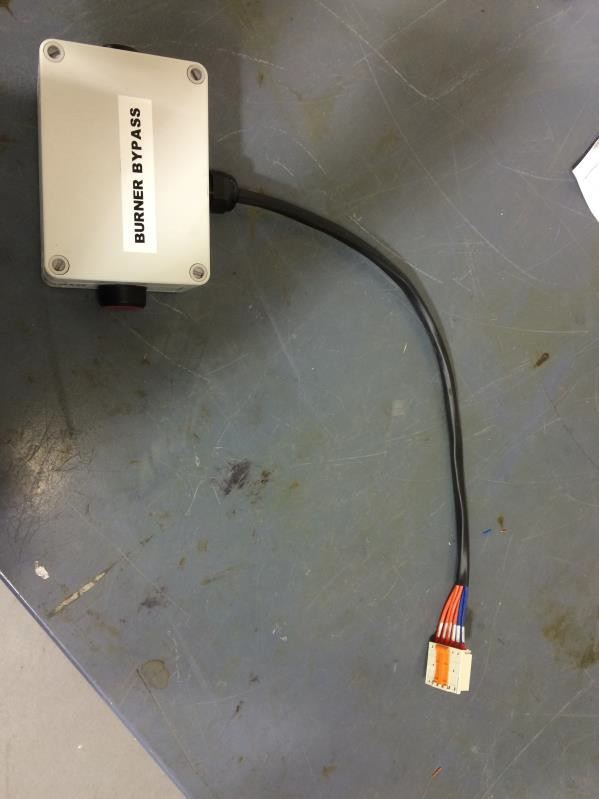
\includegraphics[width=0.8\textwidth]{pictures/burner_box/burner_box.jpg}
        \caption{Burner Bypass Box}   
        \label{fig:bypass_box}
\end{figure}

\begin{figure}[H]
        \centering
        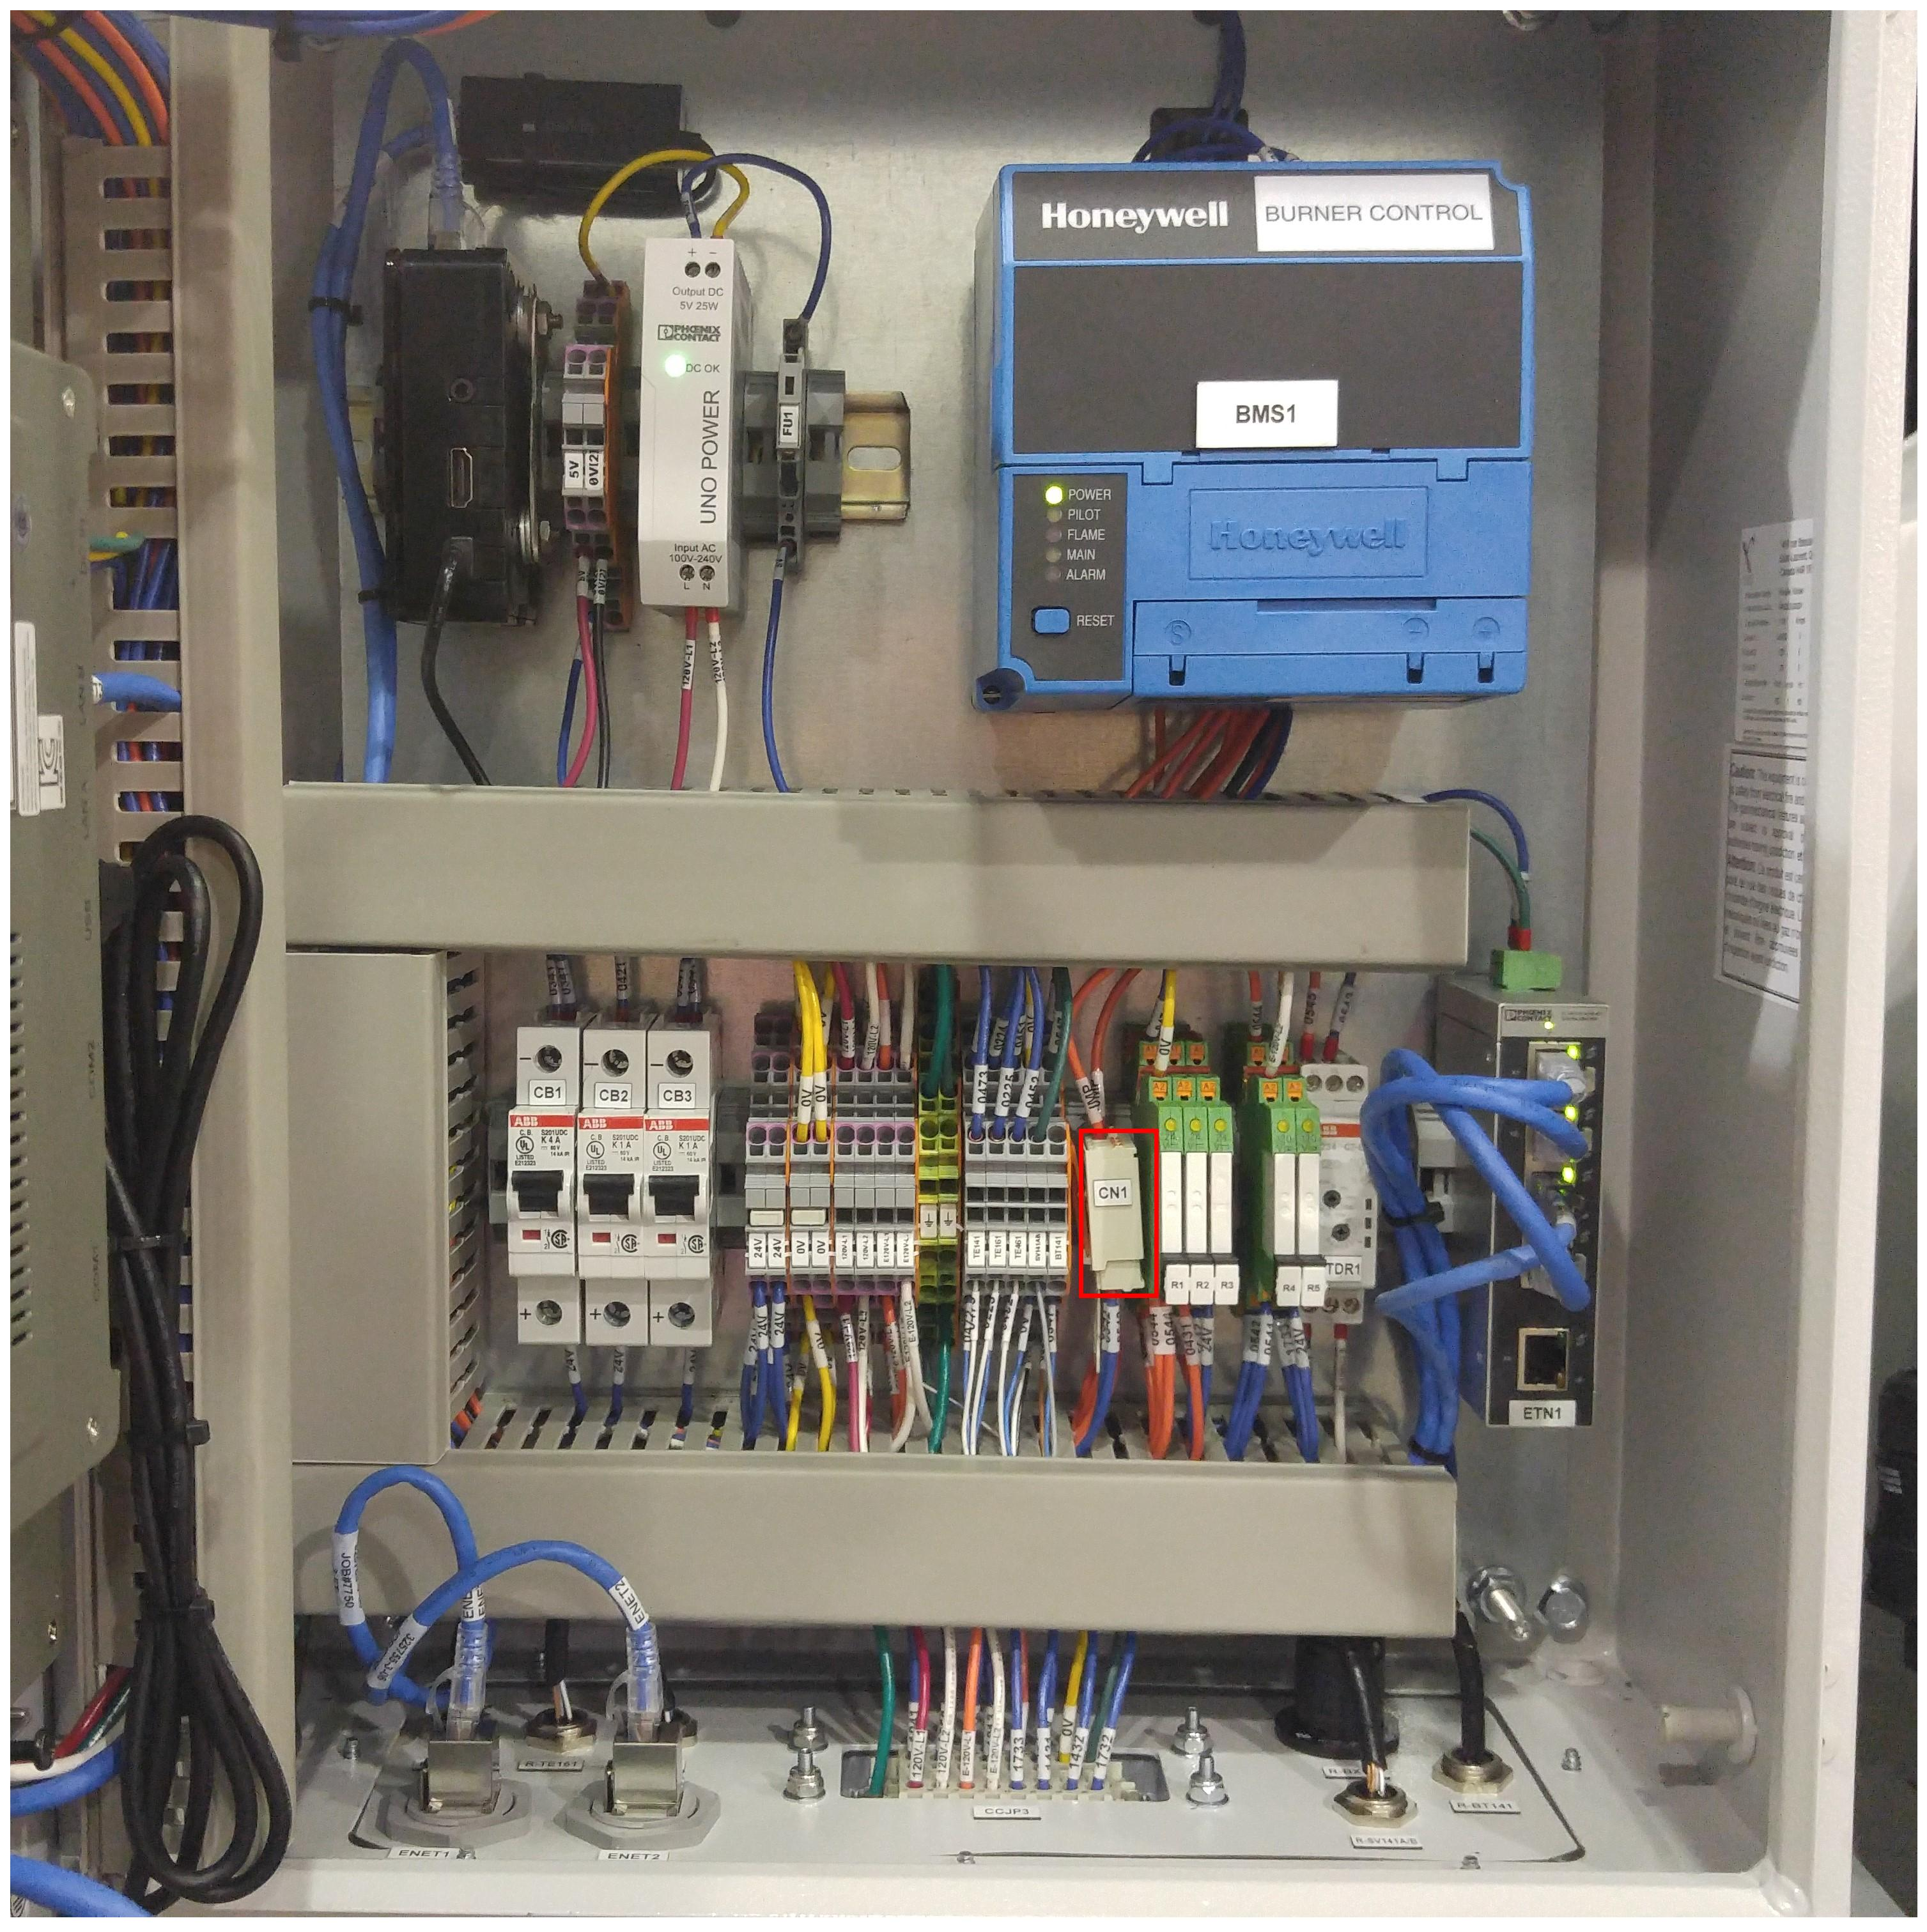
\includegraphics[width=0.8\textwidth]{pictures/burner_box/cab3_connection.jpg}
        \caption{Connection Port in CAB3}
        \label{fig:cab3_conn}
\end{figure}

\begin{figure}[H]
        \centering
        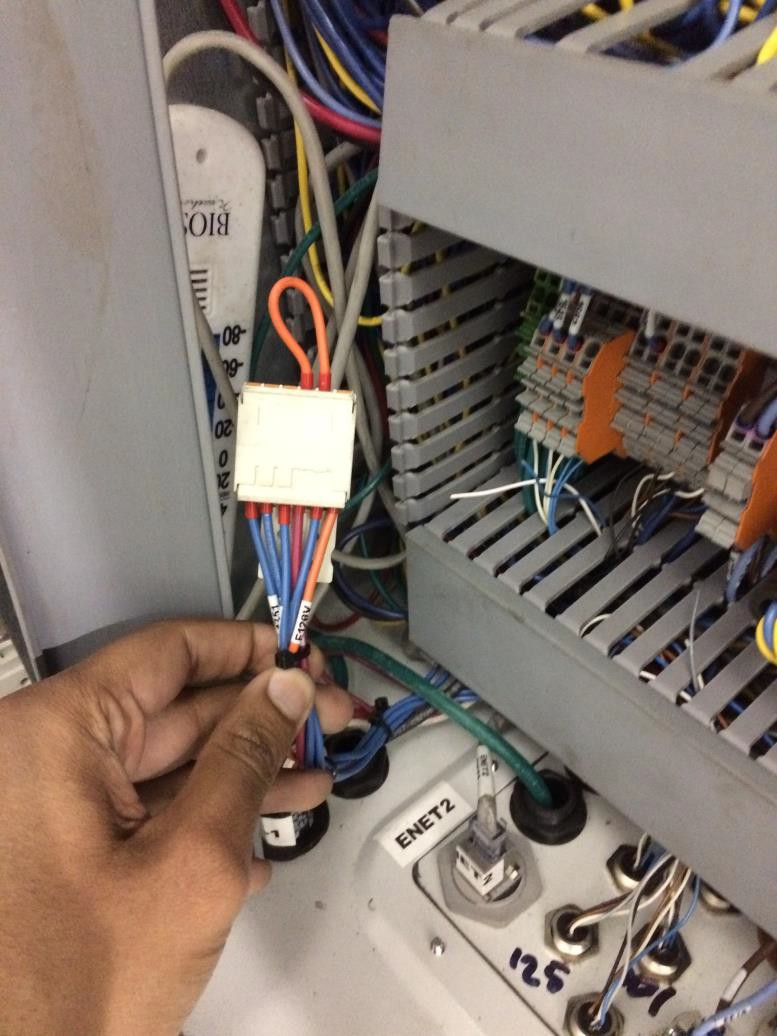
\includegraphics[width=0.8\textwidth]{pictures/burner_box/cab1_connected.jpg}
        \caption{Burner Bypass Box Connector}
        \label{fig:cab1_connector}
\end{figure}

\begin{figure}[H]
        \centering
        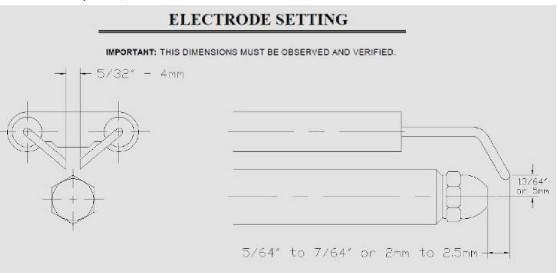
\includegraphics[width=0.8\textwidth]{pictures/burner_box/electrodes.jpg}
        \caption{Electrodes positioning}
        \label{fig:electrodes}
\end{figure}

\begin{figure}[H]
        \centering
        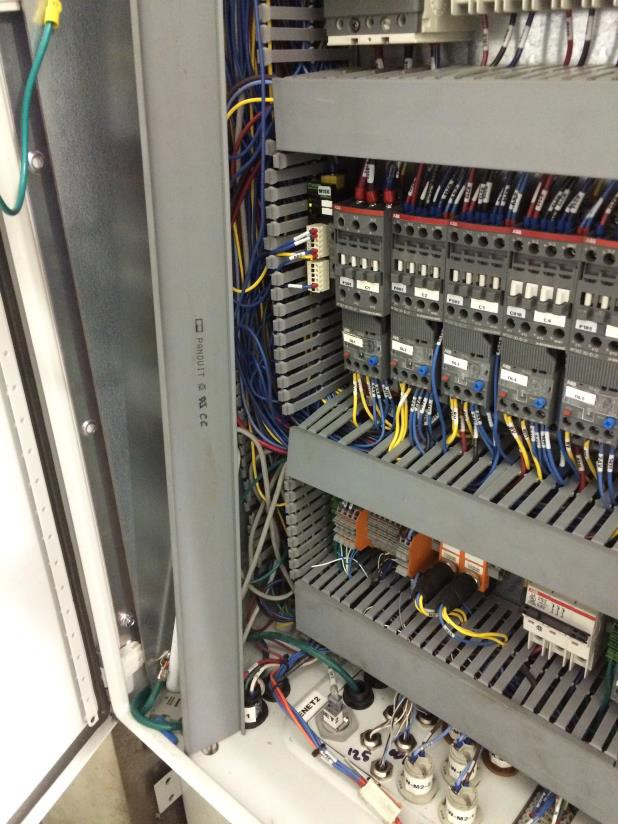
\includegraphics[width=0.8\textwidth]{pictures/burner_box/cab1_connection.jpg}
        \caption{Connection Port in CAB1}
        \label{fig:cab1_conn}
\end{figure}

\newpage
\section{Revisions}

\begin{table}[H]
    \centering
    \ra{1.3}
    \begin{tabular}{cllllll}\toprule
         \textbf{Rev} & \phantom{a} &\textbf{Changes} & \phantom{a} & \textbf{Written by} & \phantom{a} & \textbf{Date Issued} \\
        \cmidrule{3-7}
        01 & & First Issue & & Arthur Lavoie & & 18/05/2018 \\
        02 & & Added Instructions for CAB3 Connection & & Arthur Lavoie & & 06/06/2018 \\
        %& & & & & & \\
        %& & & & & & \\
        %& & & & & & \\
        %& & & & & & \\
        \bottomrule
    \end{tabular}
\end{table}

%AS-i Nodes Installation Guide
%\section{AS-i Nodes Installation}
To install AS-i nodes on a MAGS system, simply follow these steps.

\paragraph{Verify that there are no errors on the AS-i Master}.\\
On the AS-i master, make sure that the "conf/pf" for both AS-i 1 and AS-i 2 are off. If any of the two leds are on, please contact Terragon support for further debugging.

\paragraph{Install the new nodes}.\\
Start by turning off the main power from the MAGS. The new nodes have to be installed on the separator, on the left side of CAB1. Refer to the AC5211 installation guide, page 4-8. Once the node in installed, turn the power back on.

\paragraph{Update the AS-i master configuration}.\\
On the AS-i master, do the following to add the new slaves to the config: \textsc{menu} $\rightarrow$ \textsc{quick setup} $\rightarrow$ \textsc{config all}. Once completed, verify on the new slaves that the PWR and AUX leds are solid green and that all the FAULT led is off.

\paragraph{UPdate the software package and configuration file}.\\
A new software and configuration file will have to be uploaded to the HMI. Contact Terragon support for assistance.

\paragraph{Program alarm output as required}.\\
The new alarm outputs have to be configured for the desired behaviour. The settings are:
\begin{itemize}
    \item SET\_Comm\_AL002Config
    \item SET\_Comm\_AL003Config
    \item SET\_Comm\_AL004Config
    \item SET\_Comm\_AL005Config
    \item SET\_Comm\_AL006Config
    \item SET\_Comm\_AL007Config
\end{itemize}

The value for each setting is as follows:
\begin{itemize}
    \item[0:]  MAGS running Status
    \item[1:] "Cold shutdown", "Hot shutdown" or "Estop" level alarm is triggered
    \item[2:] Ready to load
    \item[3:] "Warning", "System Off", "Cold Shutdown", "Hot Shutdown" or "Estop" level alarm is triggered
    \item[4:] "System Off", "Cold Shutdown", "Hot shutdown" or "Estop" level alarm is triggered
\end{itemize}



\newpage
\section{Revisions}
\begin{table}[H]
    \centering
    \ra{1.3}
    \begin{tabular}{cllllll}\toprule
         \textbf{Rev} & \phantom{a} &\textbf{Changes} & \phantom{a} & \textbf{Written by} & \phantom{a} & \textbf{Date Issued} \\
        \cmidrule{3-7}
        01 & & First Issue & & Arthur Lavoie & & 17/01/2017 \\
        %& & & & & & \\
        %& & & & & & \\
        %& & & & & & \\
        %& & & & & & \\
        \bottomrule
    \end{tabular}
\end{table}

%Filter Swapping Quick Start Guide

\begin{minipage}{0.90\textwidth}
\begin{centering}
\wl
\textbf{
    \Large{\reporttype}\\
    \large{\rev- \release}\\
}
\end{centering}
\end{minipage}

    


\section*{First Startup}
The steps presented below will allow the user to setup the filter swapping automation to its factory setpoints.\\

Step 1: Install new bag filter in both housings.\\

Step 2: In the instruments page of the HMI, put FV503A and FV503B in manual mode; activate FV503A only. Ensure that FV407 and FV701 are not activated. Then, manually activate P503.\\

Step 3: Manually adjust the pressure release valve to 20 psi using the pressure indicator near PT503. The pressure release valve is located on the process water manifold and you should find a pressure indicator near the pressure release valve. Before turning the screw, make sure to loosen the locking nut at the base of the screw. To increase the pressure, turn the screw clockwise; to reduce it, turn the screw counter clockwise.\\

\begin{figure}[H]
        \centering
        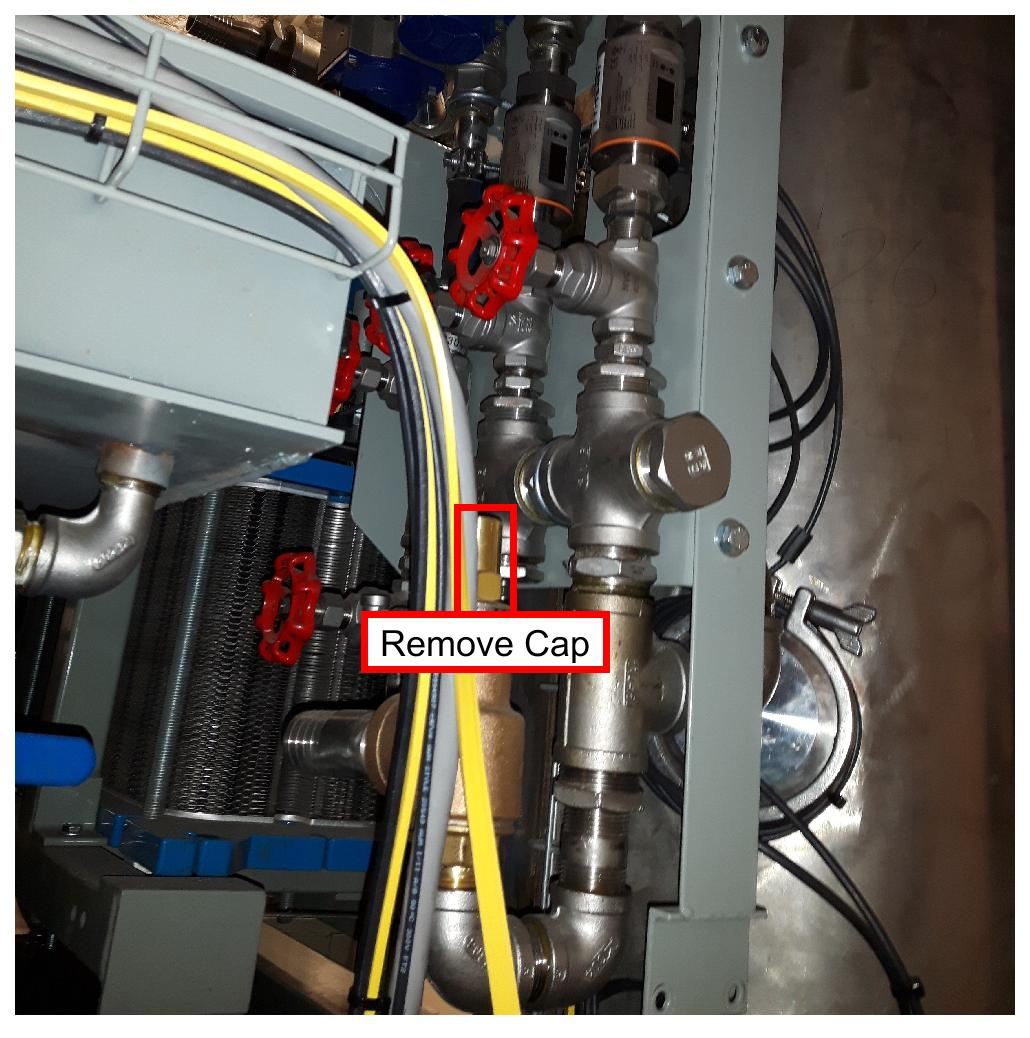
\includegraphics[width=0.45\textwidth]{pictures/filter_swap/prv_loc.jpg}
        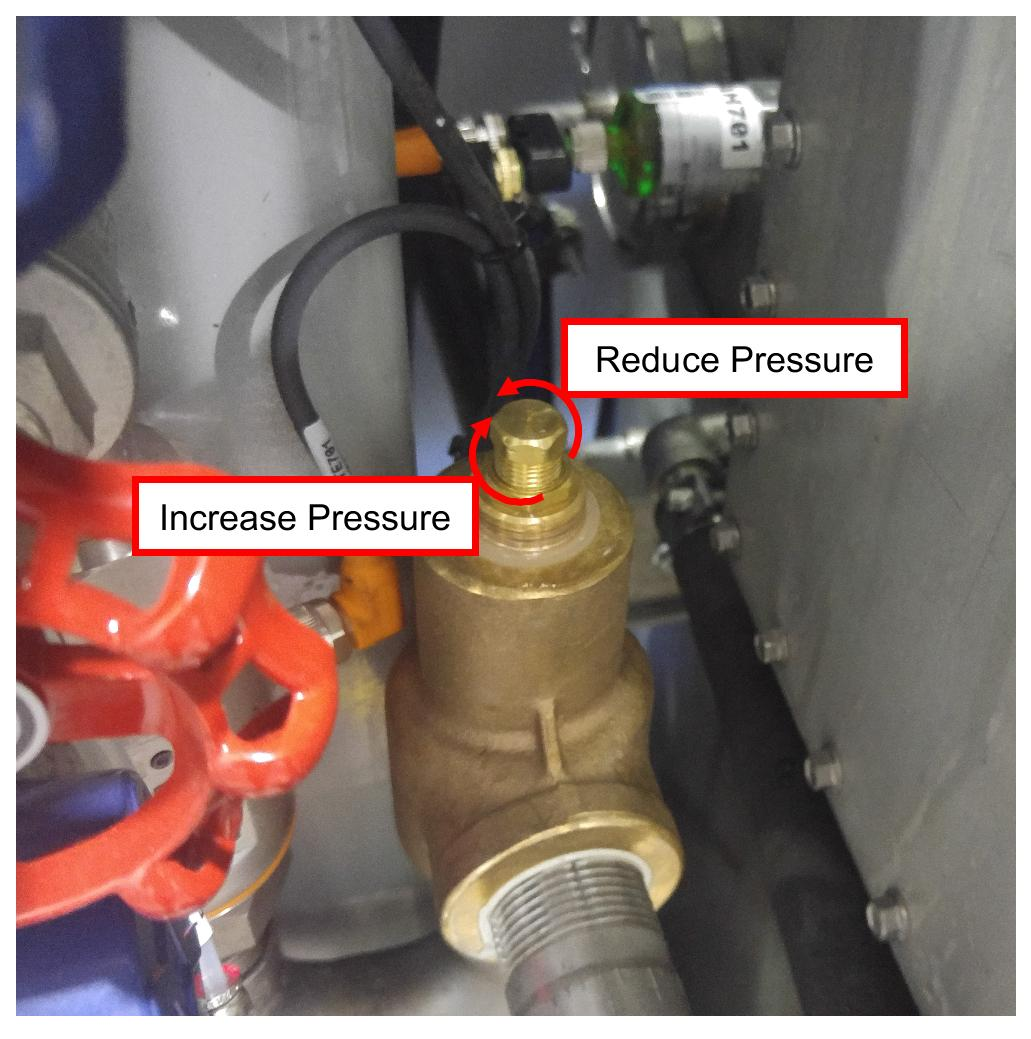
\includegraphics[width=0.45\textwidth]{pictures/filter_swap/prv_mech.jpg}
        \caption{Pressure Release Valve Adjustment}
        \label{fig:cab3_conn}
\end{figure}

Step 4: On the HMI, you should read the following values: PT503 = 20 psi and PT502 = 35 PSI.\\
\newpage
Step 5: Go to the settings page on the HMI and make sure the following settings have the values shown below:

\begin{itemize}
    \item Set\_Filter\_PT502\_NewFilter = 35 psi
    \item Set\_Filter\_PT502\_CloggedFilter = 46 psi
    \item Set\_PT502\_TrigDelay = 20 sec
    \item Set\_Filter\_PT503\_LowPressure = 10 psi
    \item Set\_Filter\_PT503\_LowPressure\_TrigDelay = 10 sec
\end{itemize}

%\newpage
\section{Revisions}

\begin{table}[H]
    \centering
    \ra{1.3}
    \begin{tabular}{cllllll}\toprule
         \textbf{Rev} & \phantom{a} &\textbf{Changes} & \phantom{a} & \textbf{Written by} & \phantom{a} & \textbf{Date Issued} \\
        \cmidrule{3-7}
        01 & & First Issue & & Arthur Lavoie & & 12/06/2018 \\
        \cmidrule{3-7}
        02 & & \begin{tabular}{@{}l@{}}Modified procedure to use P503\\ while system is stopped
        \end{tabular}  & & Arthur Lavoie & & 15/06/2018 \\
        %& & & & & & \\
        %& & & & & & \\
        %& & & & & & \\
        \bottomrule
    \end{tabular}
\end{table}

\end{document}
%%%%%%====>>>-- Fin du document --<<<====%%%%%

